\chapter{Microsoft Teams}\label{teams1}  


Introduction TODO
Petit lexique des applis de la suite Microsoft


% CONNEXION A OFFICE
\section{Connexion à Office 365 et Teams}

Ouvrez le navigateur internet de votre choix ou Safari et entrez l'URL suivante: \url{www.office.com}. Cliquez sur \textit{Connexion}.

\begin{figure}[h]
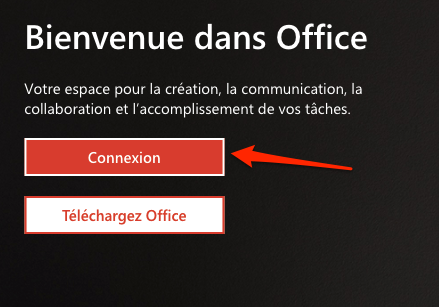
\includegraphics[width=5cm]{./images/teams/ecran_office_com_crop}
\centering
\end{figure}

Vous arrivez sur l'écran de connexion de microsoft office en ligne. Entrez votre adresse mail de l'école (qui se termine donc par \textit{@florimont.ch}).

\begin{figure}[h]
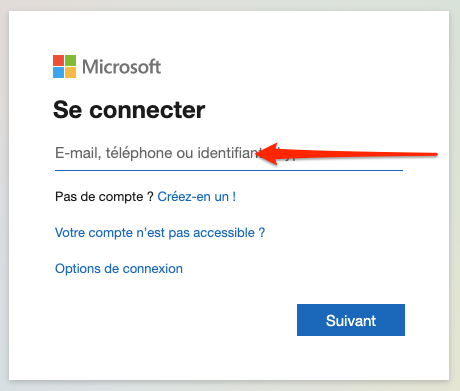
\includegraphics[width=5cm]{./images/teams/ecran_connexion_office_com_crop}
\centering
\end{figure}

Vous êtes alors redirigé vers la page d'identification de l’école. Entrez votre mot de passe. (l'adresse mail est déjà entrée, mais vous pouvez la modifier au cas où vous avez fait une erreur lors de l'étape précédente.)

\begin{figure}[h]
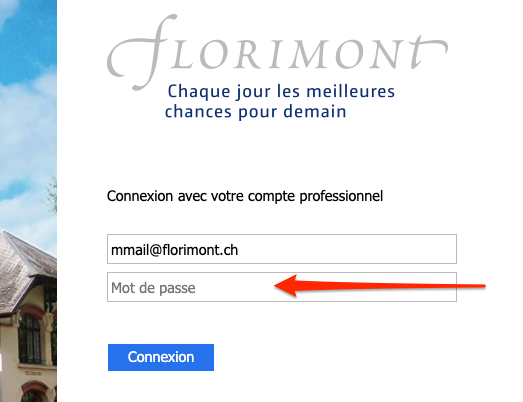
\includegraphics[width=5cm]{./images/teams/ecran_connexion_florimont_crop}
\centering
\end{figure}
\newpage
Il se peut qu'on vous demande si vous voulez rester connecté. Si vous comptez travailler longtemps sur cette session, il vaut mieux accepter.\\

En revanche, si le navigateur vous propose d'enregistrer votre mot de passe, il est recommandé de refuser (soit en fermant la fenêtre, soit en choisissant \textit{Jamais}). Si vous vous connectez depuis votre ordinateur personnel, il peut être pratique de permettre au navigateur de se souvenir de mots de passe, mais ce n'est jamais une bonne idée sur un ordinateur partagé ou d'emprunt.\\

Le site vous proposera peut-être de télécharger l’application. Cliquez alors sur \textit{Utiliser l’application web à la place}.\\

Alternativement, sur certains navigateurs (comme Safari), vous devrez télécharger l'application de bureau Teams. Cliquez sur \textit{Télécharger l'application} pour continuer.

\begin{figure}[h]
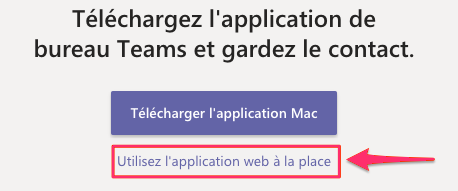
\includegraphics[width=6cm]{./images/teams/ecran_installer_teams_crop}
\centering
\end{figure}

Vous arrivez sur la page de téléchargement de l'application. Cliquez sur \textit{Download Teams}, sous le logo de la pomme, pour télécharger l'application pour Mac.\\

Vous êtes à présent dans votre espace Office. Sur la gauche, choisissez l'icône Teams.

\begin{figure}[H]
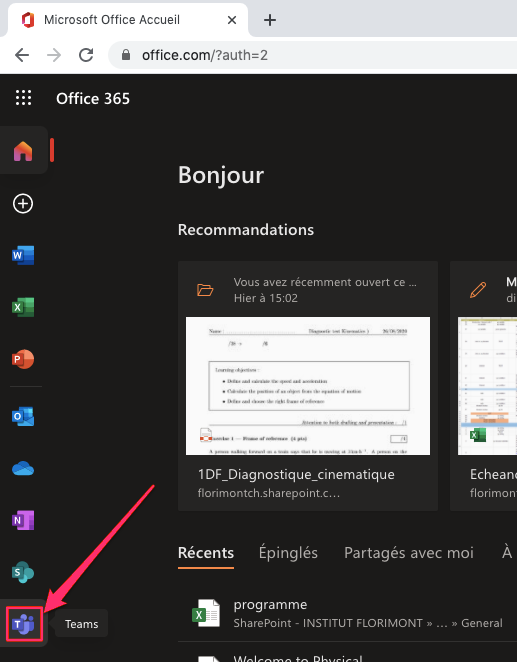
\includegraphics[width=5cm]{./images/teams/ecran_accueil_office_crop}
\centering
\end{figure}

Félicitations, vous arrivez sur la page d'accueil de votre session Teams.



% APPARENCE DE LA PAGE D'ACCUEIL
\section{Apparence de la page d'accueil}

La page d'accueil de Teams se présente sous forme d'une liste d'équipes

\begin{figure}[h]
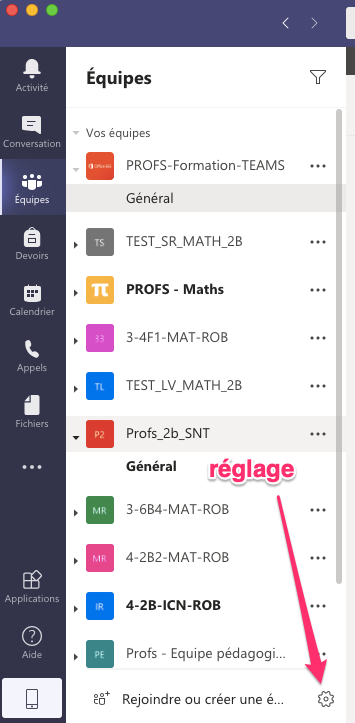
\includegraphics[width=4cm]{./images/teams/accueil_liste}
\centering
\end{figure}

ou sous forme d'une grille d'équipes 

\begin{figure}[H]
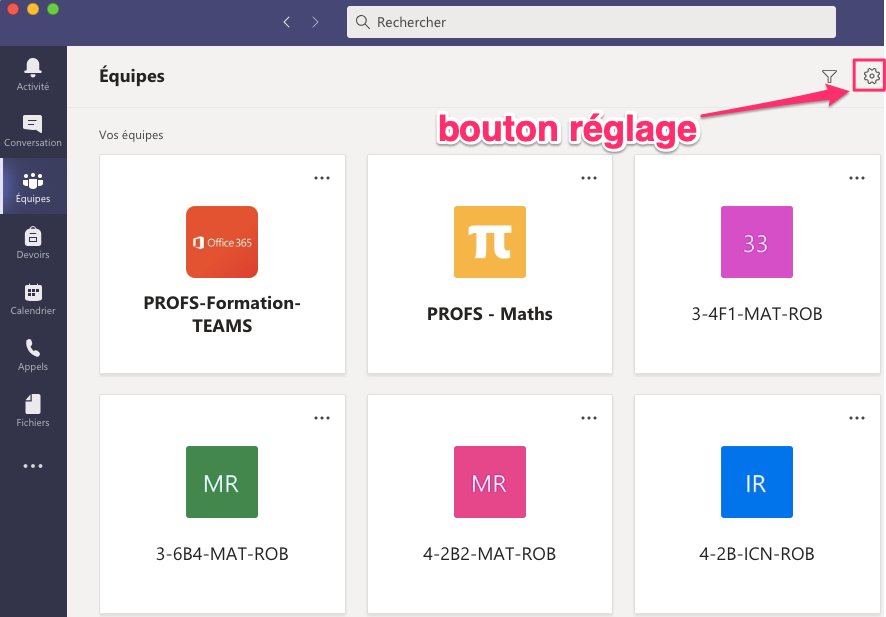
\includegraphics[width=7cm]{./images/teams/accueil_grille}
\centering
\end{figure}

Pour passer d'une forme à l'autre, il faut cliquer sur l'icône 
\includegraphics[width=0.8cm]{./images/teams/bouton_parametres}, choisir \textit{Changer d'affichage} dans le menu déroulant, comme dans l'exemple illustré ci-dessous :

\begin{figure}[h]

\includegraphics[width=8cm]{./images/teams/changement_liste}
\centering
\end{figure}

Il faut ensuite sélectionner le type d'affichage souhaité entre \textit{Grille} et \textit{Liste}

\begin{figure}[h]
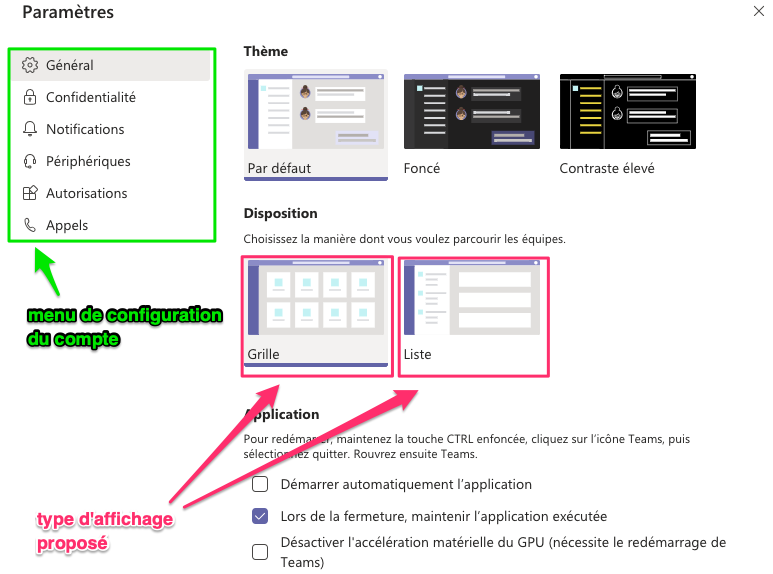
\includegraphics[width=8cm]{./images/teams/choix_parametre}
\centering
\end{figure}

 Pour entrer maintenant dans votre équipe, il suffit de cliquer sur l'icône correspondante

\begin{figure}[H]
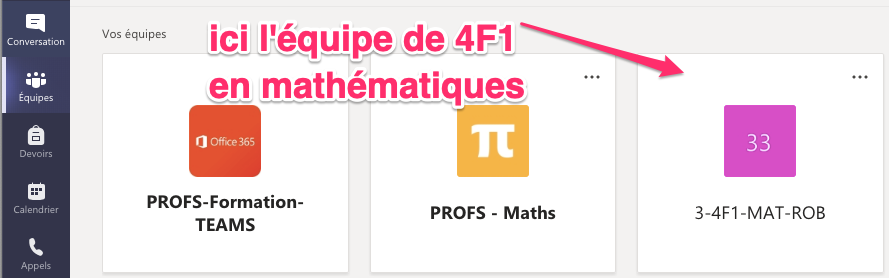
\includegraphics[width=8cm]{./images/teams/entree_classe}
\centering
\end{figure}


\newpage
% UTILISATION DE LA PUBLICATION
\section{Utilisation de la Publication}

La messagerie instantanée proposée pour chaque équipe doit permettre aux élèves et aux enseignants de communiquer en dehors de l'école dans un cadre qui reste strictement scolaire. Ainsi les messages personnels n'ont aucune raison d'être sur Teams. Il vous appartient donc de mesurer vos propos lorsque vous utilisez la messagerie instantanée. Ainsi, toute forme d'insulte ou de critique envers un membre de la classe ou une personne extérieure est à proscrire. Le modérateur de chaque équipe est son enseignant responsable.\\

Pour utiliser la messagerie, il suffit de vous rendre sur l'onglet \textit{Publications}

\begin{figure}[h]

\includegraphics[width=8cm]{./images/teams/publications}
\centering
\end{figure}

puis de rédiger du texte à l'intérieur du champ \textit{Démarrer une conversation. Utilisez @ pour mentionner un contact.}

\begin{figure}[h]
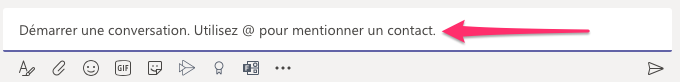
\includegraphics[width=8cm]{./images/teams/publications2}
\centering
\end{figure}

Il ne vous reste plus qu'à cliquer sur l'icône 
\includegraphics[width=0.7cm]{./images/teams/envoi_message} pour envoyer votre message.

\begin{figure}[h]
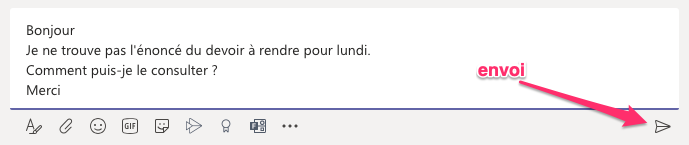
\includegraphics[width=8cm]{./images/teams/publications3}
\centering
\end{figure}





% CONSULTER ET TELECHARGER UN DOCUMENT
\section{Consulter et télécharger un document}

Nikolai

% DEPOSER UN DEVOIR
\section{Déposer un devoir}

\subsection{Consulter le sujet d'un devoir en pièce jointe}
Pour consulter les devoirs déposés par votre enseignant, il faut choisir \textit{2 de plus} dans la barre de menus du haut de page, puis sélectionner \textit{Devoirs}.\\

\begin{figure}[H]
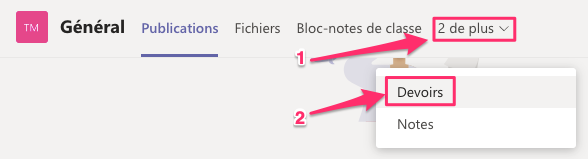
\includegraphics[width=8cm]{./images/teams/devoir1}
\centering
\end{figure}

La page qui s'affiche maintenant fait le bilan de ce qui a déjà été fait et des devoirs proposés par votre enseignant. En cliquant sur \textit{Rédaction} vous pourrez accéder au devoir.\\

\begin{figure}[h]
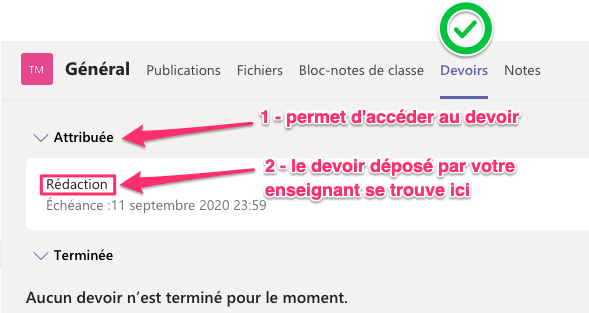
\includegraphics[width=8cm]{./images/teams/devoir2}
\centering
\end{figure}

 Vous obtenez alors l'écran suivant

\begin{figure}[h]
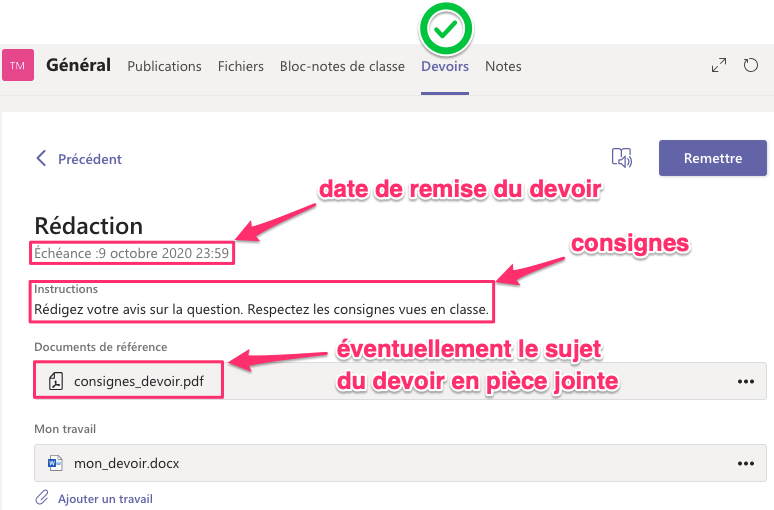
\includegraphics[width=8cm]{./images/teams/devoir3}
\centering
\end{figure}

Il est maintenant possible de consulter le sujet en sélectionnant l'icône 
\includegraphics[width=0.7cm]{./images/teams/pointilles} qui vous offre le choix entre une lecture en ligne ou un téléchargement

\begin{figure}[h]
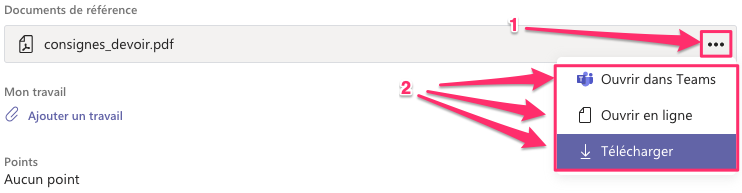
\includegraphics[width=9cm]{./images/teams/choix_pointilles}
\centering
\end{figure}

\subsection{Remettre son devoir}

Pour remettre votre devoir, il faut d'abord cliquer sur l'onglet \textit{Ajouter un travail}. S'ouvre alors une fenêtre qui vous permet de rechercher votre document sur votre ordinateur, à partir du OneDrive ou encore à partir d'une autre équipe.

\begin{figure}[H]
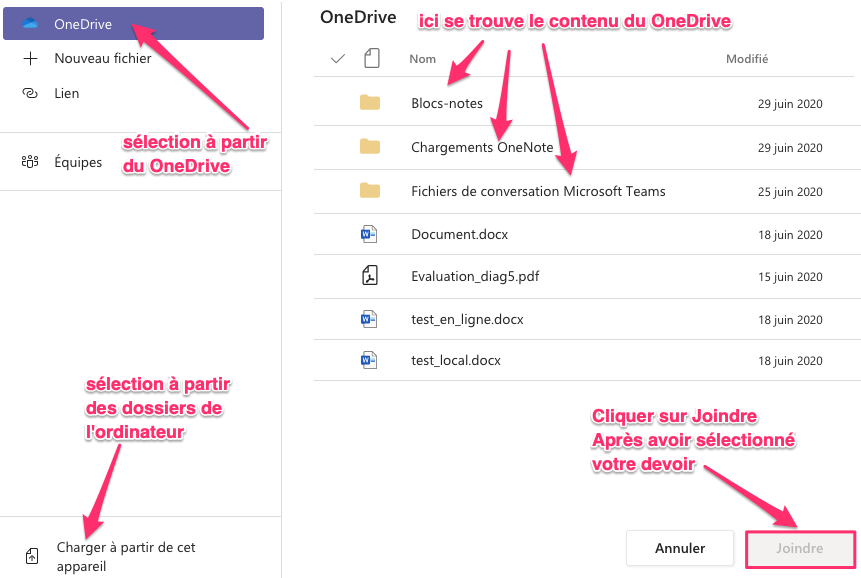
\includegraphics[width=10cm]{./images/teams/selection_devoir}
\centering
\end{figure}

Une fois votre devoir à remettre sélectionner, il suffit de cliquer sur \textit{Joindre}.\\

A ce stade, votre devoir est bien enregistré par le système, mais pas encore remis. Il faut donc choisir l'onglet \textit{Remettre} pour valider l'envoi de votre devoir.


% ACCEDER A MON CARNET
\section{Accéder à mon carnet}

Nikolai

% REJOINDRE UNE VISIO CONFERENCE
\section{Rejoindre une visio-conférence}

Steph


